% !TeX root = Bericht.tex
% !TeX spellcheck = de_DE
\section{Theorie}\label{theorie}
In diesem Kapitel wird die für die Versuchsauswertung notwendige Theorie erläutert. Hierbei wird auf die Eigenschaften von Halbleitern, den Hall-Effekt sowie auf die van-der-Pauw-Messmethode eingegangen. Der Theorieteil bezieht sich inhaltlich auf das Versuchsskript \cite{hall}.
\subsection{Hall-Effekt}
Der Hall-Effekt beschreibt das Entstehen einer elektrischen Spannung, wenn sich ein elektrischer Strom in einem stationären Magnetfeld, senkrecht auf den Stromfluss, befindet. Die entstehende Spannung steigt nicht ewig, sondern wird durch ein von der Spannung hervorgerufene elektrische Feld verringert und auf einen konstanten Wert beschränkt. Die entstehende Hall-Spannung $U_\mathrm{H}$ beträgt
\begin{equation}
    U_\mathrm{H}=R_\mathrm{H}\frac{BI}{d}.
\end{equation}
Dabei bezeichnet $B$ die Magnetfeldstärke, $I$ die angelegte Stromstärke, $d$ die Dicke der Probe und $R_\mathrm{H}$ den Hall-Koeffizienten, der später für die Auswertung essentielle Bedeutung hat.

\subsection{ Van-der-Pauw-Methode}
\label{sec:vanPauw}

Die van-der-Pauw-Methode ist eine Messmethode, um den Flächenwiderstand und den Hall-Koeffizienten eines Halbleiters zu bestimmen. Dafür wird eine Probe mit vier Anschlusspunkten A, B, C und D verwendet. Den Aufbau der Anschlusspunkte und Strom-und Spannungsmessung wird in Abbildung \ref{schaltungen} gezeigt. Zuerst wird ein elektrischer Strom $U_{\mathrm{CD}}$ zwischen A und B angelegt und die Spannung $U_{\mathrm{CD}}$ zwischen C und D gemessen. Danach werden die Anschlüsse geändert, sodass $I_{\mathrm{BC}}$ angelegt und $U_{\mathrm{DA}}$ gemessen werden kann. Daraus berechnen sich die beiden Widerstände:
\begin{equation}R_{\mathrm{AB,CD}}=\left|\frac{U_{\mathrm{CD}}}{I_{\mathrm{AB}}}\right| \quad\text{und}\quad R_{\mathrm{BC,DA}}=\left|\frac{U_{\mathrm{DA}}}{I_{\mathrm{BC}}}\right|. \end{equation}
Daraus ergibt sich der spezifische Widerstand $\rho$ als
\begin{equation}\label{eq:roh}
    \rho=\frac{\pi d}{\ln{2}}\frac{R_{\mathrm{AB,CD}}+R_{\mathrm{BC,DA}}}{2}f.
\end{equation}

Dabei ist $d$ die Dicke der Probe und $f$ ein Faktor, der  von den beiden Widerständen abhängt und durch numerisches Lösen einer transzendenten Gleichung berechnet werden kann \autocite{hall}.
\newline Dann kann der Hall Faktor $R_\mathrm{H}$ durch Anlegen des Stromes $I_\mathrm{AC}$ zwischen A und C und Messen der Spannung $U_{\mathrm{BD}}$ ermittelt werden. Der Widerstand $R_{\mathrm{AC,BD}}$ wird durch $R_{\mathrm{AC,BD}}=U_{\mathrm{BD}}/I_\mathrm{AC}$ einmal mit und einmal ohne angelegtem Magnetfeld berechnet. Dann ergibt sich der Hall Koeffizient als
\begin{equation}\label{eq:RH}
    R_\mathrm{H}=\frac{d}{B}(R_{\mathrm{AC,BD}}(B)-R_{\mathrm{AC,BD}}(0)).
\end{equation}

 \begin{figure}[H]
    \centering
    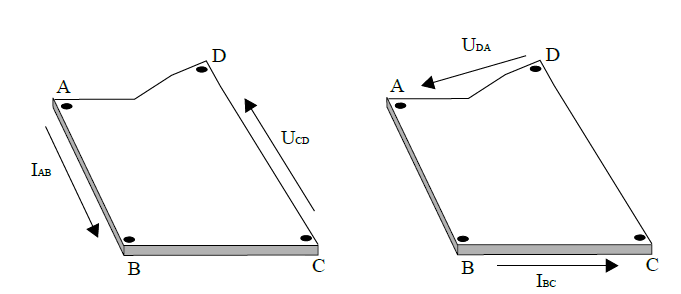
\includegraphics[ height=5cm]{vanderpauwanstecker.PNG}
    \caption{Zu sehen sind eine symbolische Probe sowie die vier Anschlusspunkte A, B, C und D, die nach der van der Pauw Methode angeschlossen werden.\cite{hall}}
   \label{schaltungen}
\end{figure}
Abbildung \ref{schaltungen_vdp} zeigt alle möglichen Kombinationen des Anlegens der Stromstärke und Messung der Spannung, wobei diese Schaltungen in unserem Versuchsaufbau mit einem Drehschalter realisiert werden, dessen Optionen als Konfiguration bezeichnet werden.
 \begin{figure}[H]
    \centering
    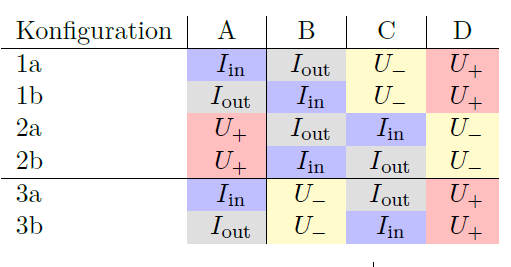
\includegraphics[ height=5cm]{tabelle_drehen.PNG}
    \caption{Zu sehen sind die möglichen Konfigurationen am Drehschalter mit deren zugehörigen Schaltungen.\cite{hall} }
   \label{schaltungen_vdp}
\end{figure}
\subsection{Beweglichkeit der Ladungsträger und Leitfähigkeit}
Mithilfe des Hall Koeffizienten lässt sich die Ladungsträgerdichte der Elektronen bzw. Löcher, n bzw. p, ermitteln als:
\begin{equation}\label{eq:RHn}
    R_{\mathrm{H}}^{(\mathrm{n})}=-\frac{1}{e n} \quad\text{ bzw. }\quad R_{\mathrm{H}}^{(\mathrm{p})}=\frac{1}{e p}.
\end{equation}

Daraus lässt sich die Beweglichkeit  der negativ geladenen Ladungsträger $\mu_{\mathrm{n}}$ bestimmen:
\begin{equation}\label{eq:mu}
    \mu_{\mathrm{n}}=\frac{R_{\mathrm{H}}}{\rho}.
\end{equation}
Die Formel für p-Dotierung sieht äquivalent aus.
Die Leitfähigkeit $\sigma$ wird als Kehrwert des spezifischen Widerstands $\rho$ bestimmt als $\sigma=\rho^{-1}$.


\subsection{Streuung und Matthiessensche Regel}
\label{sec:Streuung}
Abhängig von der Temperatur ändert sich die dominierende Streuungsart im Halbleiter. Bei niedrigen Temperaturen findet hauptsächlich elastische Streuung geladener Teilchen (Rutherford-Streuung) statt. Für die Relaxationszeit $\tau$, die mittlere Zeit zwischen zwei Stößen, ergibt sich die Proportionalität $\tau_{\mathrm{Ion}}\propto T^{3/2} $, wobei $T$ die Temperatur ist.
Für hohe Temperaturen wird hauptsächlich Streuung an Phononen, also Gitterschwingungen, beobachtet. Für diese Art ergibt sich der Zusammenhang $\tau_{\mathrm{Ph}}\propto T^{-3/2}$. \newline
Die Matthiessensche Regel beschreibt die effektive Relaxationszeit $\tau$ bei mehreren Stoßprozessen, diese ergibt sich als
\begin{equation}
    \frac{1}{\tau}=\sum_i \frac{1}{\tau_{\mathrm{i}}}.
\end{equation}
\subsection{Intrinsischer und extrinsischer Halbleiter}
Die intrinsische Leitfähigkeit eines Halbleiters ist die Leitfähigkeit ohne Dotierung und entsteht bei Anregung von Elektronen über die Bandlücke. Dies geschieht nur bei hohen Temperaturen ($T > 300 \unit{K}$). Für die intrinsische Ladungsträgerdichte $n_\mathrm{i}$ gilt
\begin{equation}
    n_{\mathrm{i}}=p_{\mathrm{i}}=
    \sqrt{N_{\mathrm{L}}N_{\mathrm{V}}}
    \exp{\left[-\frac{E_{\mathrm{G}}}{2k_{\mathrm{B}}T}\right]}.
\end{equation}

Wenn hingegen die Störstellen die Leitfähigkeit dominieren, spricht man vom extrinsischen Halbleiter. Hier unterscheidet man zwei Möglichkeiten.

Bei einer Temperatur, die Ionisation aller Störstellen erreicht, aber zu gering ist, um Elektron-Loch-Paare zu erzeugen, wird die Ladungsträgerdichte durch die Störstellendichte der Donatoren $N_{\mathrm{D}}$ bzw. Akzeptoren $N_{\mathrm{A}}$ bestimmt. Für eine n-Dotierung gilt näherungsweise $n \approx N_{\mathrm{D}}=const.$, für eine p-Dotierung $p \approx N_{\mathrm{A}}=const.$.

Ist die Temperatur zu tief, um alle Störstellen zu ionisieren, gilt für die Ladungsträgerdichte:
\begin{equation}
    n=\sqrt{N_{\mathrm{D}}N_{\mathrm{V}}}\exp{\left[-\frac{E_{\mathrm{d}}}{2k_{\mathrm{B}T}}\right]}.
\end{equation}\label{eq:Ed}
Dabei bezeichnet $E_{\mathrm{D}}$ das Energieniveau der Donatoren, und $E_{\mathrm{d}}=E_{\mathrm{D}}-E_{\mathrm{L}}$ die Ionisierungsenergie. Dieser Zusammenhang wird mithilfe eines logarithmischen Plots von $\ln(n)$ verwendet, um die Ionsierungsenergie durch einen Fit zu bestimmen. Die Größe $N_{\mathrm{V}}$ bezeichnet die Dichte der Ladungsträger am Valenzband.


